%%%%%%%%%%%%%%%%%%%%%%%%%%%%%%%%%%%%%%%%%%%%%%%%%%%%%%%%%%%%%%%%%%%%%%%%%%%%%%%%
% Template for USENIX papers.
%
% History:
%
% - TEMPLATE for Usenix papers, specifically to meet requirements of
%   USENIX '05. originally a template for producing IEEE-format
%   articles using LaTeX. written by Matthew Ward, CS Department,
%   Worcester Polytechnic Institute. adapted by David Beazley for his
%   excellent SWIG paper in Proceedings, Tcl 96. turned into a
%   smartass generic template by De Clarke, with thanks to both the
%   above pioneers. Use at your own risk. Complaints to /dev/null.
%   Make it two column with no page numbering, default is 10 point.
%
% - Munged by Fred Douglis <douglis@research.att.com> 10/97 to
%   separate the .sty file from the LaTeX source template, so that
%   people can more easily include the .sty file into an existing
%   document. Also changed to more closely follow the style guidelines
%   as represented by the Word sample file.
%
% - Note that since 2010, USENIX does not require endnotes. If you
%   want foot of page notes, don't include the endnotes package in the
%   usepackage command, below.
% - This version uses the latex2e styles, not the very ancient 2.09
%   stuff.
%
% - Updated July 2018: Text block size changed from 6.5" to 7"
%
% - Updated Dec 2018 for ATC'19:
%
%   * Revised text to pass HotCRP's auto-formatting check, with
%     hotcrp.settings.submission_form.body_font_size=10pt, and
%     hotcrp.settings.submission_form.line_height=12pt
%
%   * Switched from \endnote-s to \footnote-s to match Usenix's policy.
%
%   * \section* => \begin{abstract} ... \end{abstract}
%
%   * Make template self-contained in terms of bibtex entires, to allow
%     this file to be compiled. (And changing refs style to 'plain'.)
%
%   * Make template self-contained in terms of figures, to
%     allow this file to be compiled. 
%
%   * Added packages for hyperref, embedding fonts, and improving
%     appearance.
%   
%   * Removed outdated text.
%
%%%%%%%%%%%%%%%%%%%%%%%%%%%%%%%%%%%%%%%%%%%%%%%%%%%%%%%%%%%%%%%%%%%%%%%%%%%%%%%%

\documentclass[letterpaper,twocolumn,10pt]{article}
\usepackage{usenix-2020-09}

% for urls
\usepackage{hyperref}

% to be able to draw some self-contained figs
\usepackage{tikz}
\usepackage{amsmath}

% inlined bib file
\usepackage{filecontents}

%-------------------------------------------------------------------------------
\begin{filecontents}{\jobname.bib}
%-------------------------------------------------------------------------------
@misc{gu20ropriscv,
    title={{Return}-{Oriented} {Programming} in {RISC-V}},
    author={Gu, Garrett and Shacham, Hovav},
    year={2020},
    eprint={2007.14995},
    archivePrefix={arXiv},
    primaryClass={cs.CR},
}
@inproceedings{bletsch11jopx86,
    author = {Bletsch, Tyler and Jiang, Xuxian and Freeh, Vince W. and Liang, Zhenkai},
    title = {{Jump}-{Oriented} {Programming}: {A} {New} {Class} of {Code}-{Reuse} {Attack}},
    year = {2011},
    isbn = {9781450305648},
    publisher = {Association for Computing Machinery},
    address = {New York, NY, USA},
    url = {https://doi.org/10.1145/1966913.1966919},
    doi = {10.1145/1966913.1966919},
    abstract = {Return-oriented programming is an effective code-reuse attack in which short code sequences ending in a ret instruction are found within existing binaries and executed in arbitrary order by taking control of the stack. This allows for Turing-complete behavior in the target program without the need for injecting attack code, thus significantly negating current code injection defense efforts (e.g., W⊕X). On the other hand, its inherent characteristics, such as the reliance on the stack and the consecutive execution of return-oriented gadgets, have prompted a variety of defenses to detect or prevent it from happening.In this paper, we introduce a new class of code-reuse attack, called jump-oriented programming. This new attack eliminates the reliance on the stack and ret instructions (including ret-like instructions such as pop+jmp) seen in return-oriented programming without sacrificing expressive power. This attack still builds and chains functional gadgets, each performing certain primitive operations, except these gadgets end in an indirect branch rather than ret. Without the convenience of using ret to unify them, the attack relies on a dispatcher gadget to dispatch and execute the functional gadgets. We have successfully identified the availability of these jump-oriented gadgets in the GNU libc library. Our experience with an example shellcode attack demonstrates the practicality and effectiveness of this technique.},
    booktitle = {Proceedings of the 6th ACM Symposium on Information, Computer and Communications Security},
    pages = {30–40},
    numpages = {11},
    location = {Hong Kong, China},
    series = {ASIACCS '11}
}
@inproceedings{shacham07ropx86,
    author = {Shacham, Hovav},
    title = {{The} {Geometry} of {Innocent} {Flesh} on the {Bone}: {Return}-into-{Libc} without {Function} {Calls} (on the {X86})},
    year = {2007},
    isbn = {9781595937032},
    publisher = {Association for Computing Machinery},
    address = {New York, NY, USA},
    url = {https://doi.org/10.1145/1315245.1315313},
    doi = {10.1145/1315245.1315313},
    abstract = {We present new techniques that allow a return-into-libc attack to be mounted on x86 executables that calls no functions at all. Our attack combines a large number of short instruction sequences to build gadgets that allow arbitrary computation. We show how to discover such instruction sequences by means of static analysis. We make use, in an essential way, of the properties of the x86 instruction set.},
    booktitle = {Proceedings of the 14th ACM Conference on Computer and Communications Security},
    pages = {552–561},
    numpages = {10},
    keywords = {return-into-libc, instruction set, turing completeness},
    location = {Alexandria, Virginia, USA},
    series = {CCS '07}
}
@inproceedings{patterson98risc,
    title={{RISC} {I}: {A} reduced instruction set {VLSI} computer},
    author={Patterson, David A and Sequin, Carlo H},
    booktitle={25 years of the international symposia on Computer architecture (selected papers)},
    pages={216--230},
    year={1998}
}
@inproceedings{checkoway10ropnoret,
    author = {Checkoway, Stephen and Davi, Lucas and Dmitrienko, Alexandra and Sadeghi, Ahmad-Reza and Shacham, Hovav and Winandy, Marcel},
    title = {{Return}-{Oriented} {Programming} without {Returns}},
    year = {2010},
    isbn = {9781450302456},
    publisher = {Association for Computing Machinery},
    address = {New York, NY, USA},
    url = {https://doi.org/10.1145/1866307.1866370},
    doi = {10.1145/1866307.1866370},
    abstract = {We show that on both the x86 and ARM architectures it is possible to mount return-oriented programming attacks without using return instructions. Our attacks instead make use of certain instruction sequences that behave like a return, which occur with sufficient frequency in large libraries on (x86) Linux and (ARM) Android to allow creation of Turing-complete gadget sets.Because they do not make use of return instructions, our new attacks have negative implications for several recently proposed classes of defense against return-oriented programming: those that detect the too-frequent use of returns in the instruction stream; those that detect violations of the last-in, first-out invariant normally maintained for the return-address stack; and those that modify compilers to produce code that avoids the return instruction.},
    booktitle = {Proceedings of the 17th ACM Conference on Computer and Communications Security},
    pages = {559–572},
    numpages = {14},
    keywords = {return-oriented programming, arm, x86},
    location = {Chicago, Illinois, USA},
    series = {CCS '10}
}
@inproceedings{sadeghi15tinyjop,
    author = {Sadeghi, Ali-Akbar and Aminmansour, Farzane and Shahriari, Hamid-Reza},
    year = {2015},
    month = {09},
    pages = {52-57},
    title = {{Tiny} jump-oriented programming attack ({A} class of code reuse attacks)},
    doi = {10.1109/ISCISC.2015.7387898}
}
@inbook{jaloyan20ropriscv,
    author = {Jaloyan, Georges-Axel and Markantonakis, Konstantinos and Akram, Raja Naeem and Robin, David and Mayes, Keith and Naccache, David},
    title = {{Return}-{Oriented} {Programming} on {RISC-V}},
    year = {2020},
    isbn = {9781450367509},
    publisher = {Association for Computing Machinery},
    address = {New York, NY, USA},
    url = {https://doi.org/10.1145/3320269.3384738},
    abstract = {This paper provides the first analysis on the feasibility of Return-Oriented programming (ROP) on RISC-V, a new instruction set architecture targeting embedded systems. We show the existence of a new class of gadgets, using several Linear Code Sequences And Jumps (LCSAJ), undetected by current Galileo-based ROP gadget searching tools. We argue that this class of gadgets is rich enough on RISC-V to mount complex ROP attacks, bypassing traditional mitigation like DEP, ASLR, stack canaries, G-Free and some compiler-based backward-edge CFI, by jumping over any guard inserted by a compiler to protect indirect jump instructions. We provide examples of such gadgets, as well as a proof-of-concept ROP chain, using C code injection to leverage a privilege escalation attack on two standard Linux operating systems. Additionally, we discuss some of the required mitigations to prevent such attacks and provide a new ROP gadget finder algorithm that handles this new class of gadgets.},
    booktitle = {Proceedings of the 15th ACM Asia Conference on Computer and Communications Security},
    pages = {471–480},
    numpages = {10}
}
@manual{riscvmanual,
    author = {Waterman, Andrew and Asanovic, Krste},
    title = {{The} {RISC-V} {Instruction} {Set} {Manual}, {Volume} {I}: {User}-{Level} {ISA}, {Document} {Version} {20191213}},
    note = {\url{https://github.com/riscv/riscv-isa-manual}}
}
@inproceedings{fixer,
    author={A. {De} and A. {Basu} and S. {Ghosh} and T. {Jaeger}},
    booktitle={2019 Design, Automation   Test in Europe Conference   Exhibition (DATE)}, 
    title={FIXER: Flow Integrity Extensions for Embedded RISC-V}, 
    year={2019},
    volume={},
    number={},
    pages={348-353},
    doi={10.23919/DATE.2019.8714980}
}
@misc{zipper,
      title={Zipper Stack: Shadow Stacks Without Shadow}, 
      author={Jinfeng Li and Liwei Chen and Qizhen Xu and Linan Tian and Gang Shi and Kai Chen and Dan Meng},
      year={2020},
      eprint={1902.00888},
      archivePrefix={arXiv},
      primaryClass={cs.CR}
}


\end{filecontents}

%-------------------------------------------------------------------------------
\begin{document}
%-------------------------------------------------------------------------------

%don't want date printed
\date{}

% make title bold and 14 pt font (Latex default is non-bold, 16 pt)
\title{\Large \bf JOP in RISC-V:\\
  (working title)}

%for single author (just remove % characters)
\author{
{\rm Daniel Starikov}\\
Univeristy of Washington
\and
{\rm Keanu Vestil}\\
University of Washington
% copy the following lines to add more authors
% \and
% {\rm Name}\\
%Name Institution
} % end author

\maketitle

%-------------------------------------------------------------------------------
\begin{abstract}
%-------------------------------------------------------------------------------
Your abstract text goes here. Just a few facts. Whet our appetites.
Not more than 200 words, if possible, and preferably closer to 150.
\end{abstract}


%-------------------------------------------------------------------------------
\section{Introduction}
%-------------------------------------------------------------------------------

RISC-V is a free and open instruction set architecture (ISA) introduced by UC
Berkeley in 2010. Although it was initially designed for research and education
purposes, it is being increasingly used in commercial settings. RISC-V is a
based on the reduced instruction set computer (RISC) paradigm. This aims to
improve a machine's throughput by simplifying instructions and addressing modes,
thus reducing the cycles needed per instruction and reducing the time per cycle~\cite{patterson98risc}.

[paragraph about code reuse attacks]

[paragraph about ROP and JOP]

[paragraph about]

%-------------------------------------------------------------------------------
\section{Implementing Variations of ROP}
%-------------------------------------------------------------------------------

We thought it would be beneficial to recreate previously demonstrated ROP attacks
so that we could familiarize ourselves with the process. We began by testing the
RISC-V ROP attack described in Gu and Shacham~\cite{gu20ropriscv}. We cloned
their publicly available GitHub repository to our machine and successfully
replicated their ROP attack on our RISC-V VM. To replicate their attack on our VM, we
found the exact version of \verb|libc.so| that the authors used and cross-referenced
it with the addresses from their compiler to find their exact gadgets. We then
implemented these gadgets in an assembly file and modified their compiler to use
the addresses of our gadgets. With this in place we were able to successfully execute
brainfuck programs through ROP on our VM's. Next we sought to port a variant of
ROP, which does not use returns~\cite{checkoway10ropnoret}, from x86 to RISC-V.

At first, we reused the gadgets that we implemented in the aforementioned plain ROP
attack. Instead of loading the return address into \verb|ra|, we modified the
gadgets to load it into \verb|a6|. The \verb|ret| and \verb|jalr ra|
instructions at the end of each gadget were replaced with \verb|c.jalr a6|.
Since \verb|a6| was otherwise unused in our gadgets, this functionality is
effectively the same as normal behavior with the exception that the \verb|ret|
and \verb|jalr ra| mnemonics are never used. This was a successful proof of
concept, but it was not realistic because it relied on gadget modification that
we manufactured.

Checkoway et al. described a ``trampoline'' gadget that could be reused to
achieve this \verb|ret|-like behavior. We were able to successfully implement
a simplified version of this attack using a real \verb|ret| gadget which incremented
the stack pointer and performed a ret, allowing us to reuse the JOP versions of ROP gadgets that
relied on loading from the stack. We modified our gadgets ending with \verb|c.jalr a6|
to no longer modify the stack pointer. We then rewrote the brainfuck to ROP compiler
from \cite{gu20ropriscv} to use our updated JOP gadgets and chained them together
using the new \verb|ret| gadget. Finally, we demonstrated that this could extend to a
full ROP-without-returns attack by replacing the real \verb|ret| gadget with one
that we wrote ourselves which increments the stack pointer and ends with an indirect jump.
This attack is also not realistic as it relies on the modified gadgets that use the stack
and requires an unrealistic gadget that increments the stack before performing an indirect jump.

Footnotes should be places after punctuation characters, without any
spaces between said characters and footnotes, like so.%
\footnote{Remember that USENIX format stopped using endnotes and is
  now using regular footnotes.} And some embedded literal code may
look as follows.

\begin{verbatim}
int main(int argc, char *argv[]) 
{
    return 0;
}
\end{verbatim}

This is an example citation of Gu and Shacham~\cite{gu20ropriscv}. This is an
example of citing two papers at once, which both discuss x86-based code reuse
attacks~\cite{shacham07ropx86,bletsch11jopx86}.

The tilde character (\~{}) in the tex source means a non-breaking
space. This way, your reference will always be attached to the word
that preceded it, instead of going to the next line.

And the 'cite' package sorts your citations by their numerical order
of the corresponding references at the end of the paper.

It'd be nice and thoughtful of you to include a suitable link in each
and every bibtex entry that you use in your submission, to allow
reviewers (and other readers) to easily get to the cited work.

Now we're going take a look at Section~\ref{sec:figs}, but not before
observing that refs to sections and citations and such are colored and
clickable in the PDF because of the packages we've included.

%-------------------------------------------------------------------------------
\section{Floating Figures and Lists}
\label{sec:figs}
%-------------------------------------------------------------------------------


%---------------------------
\begin{figure}
\begin{center}
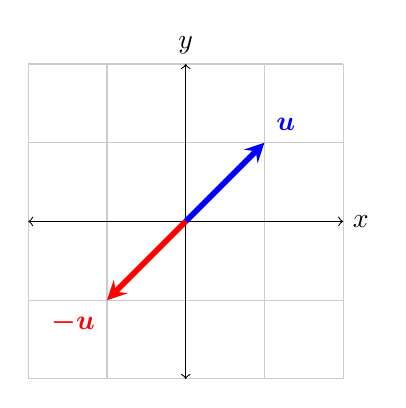
\begin{tikzpicture}
  \draw[thin,gray!40] (-2,-2) grid (2,2);
  \draw[<->] (-2,0)--(2,0) node[right]{$x$};
  \draw[<->] (0,-2)--(0,2) node[above]{$y$};
  \draw[line width=2pt,blue,-stealth](0,0)--(1,1)
        node[anchor=south west]{$\boldsymbol{u}$};
  \draw[line width=2pt,red,-stealth](0,0)--(-1,-1)
        node[anchor=north east]{$\boldsymbol{-u}$};
\end{tikzpicture}
\end{center}
\caption{\label{fig:vectors} Text size inside figure should be as big as
  caption's text. Text size inside figure should be as big as
  caption's text. Text size inside figure should be as big as
  caption's text. Text size inside figure should be as big as
  caption's text. Text size inside figure should be as big as
  caption's text. }
\end{figure}
%% %---------------------------


Here's a typical reference to a floating figure:
Figure~\ref{fig:vectors}. Floats should usually be placed where latex
wants then. Figure\ref{fig:vectors} is centered, and has a caption
that instructs you to make sure that the size of the text within the
figures that you use is as big as (or bigger than) the size of the
text in the caption of the figures. Please do. Really.

In our case, we've explicitly drawn the figure inlined in latex, to
allow this tex file to cleanly compile. But usually, your figures will
reside in some file.pdf, and you'd include them in your document
with, say, \textbackslash{}includegraphics.

Lists are sometimes quite handy. If you want to itemize things, feel
free:

\begin{description}
  
\item[fread] a function that reads from a \texttt{stream} into the
  array \texttt{ptr} at most \texttt{nobj} objects of size
  \texttt{size}, returning returns the number of objects read.

\item[Fred] a person's name, e.g., there once was a dude named Fred
  who separated usenix.sty from this file to allow for easy
  inclusion.
\end{description}

\noindent
The noindent at the start of this paragraph in its tex version makes
it clear that it's a continuation of the preceding paragraph, as
opposed to a new paragraph in its own right.


\subsection{LaTeX-ing Your TeX File}
%-----------------------------------

People often use \texttt{pdflatex} these days for creating pdf-s from
tex files via the shell. And \texttt{bibtex}, of course. Works for us.

%-------------------------------------------------------------------------------
\section{Implementing JOP}
%-------------------------------------------------------------------------------

In this section we describe our methodology for crafting a jump-oriented
programming attack. In addition, we discuss its capabilities, limitations, and
possible real-world applications. Our approach is inspired by the previous work
on this topic by Bletsch et al.~\cite{bletsch11jopx86}. Their research was done
on x86, so part of our work was to translate their results to work in RISC-V. In
their findings, they describe a \textit{dispatcher} gadget and an
\textit{initializer} gadget. A dispatcher gadget increments a register that is
used as a pseudo-program counter and then jumps to the address stored at that
next address. An initializer gadget loads many (or perhaps all) registers that
the proceeding gadgets rely on. In x86, the \verb|popa| instruction loads every
general purpose register from the stack. There is no such luxury in RISC-V, but
we found a gadget that achieves a similar effect.

There is a powerful initializer gadget in the \verb|setcontext| function from
\verb|libc|. It loads almost all%
% TODO: \verb| | the registers in this foonote, somehow
\footnote{gp, tp, t0, t2 are the only registers that are not set by this
initializer gadget.}
general purpose registers from memory, based on the address in the \verb|t0|
register, and then it jumps to the address that it just loaded into \verb|t1|.
The ability to load so many register from memory and to subsequently jump to an
address that we can arbitrarily define makes this gadget quite versatile.
However, before we can utilize it, we must set \verb|t0| to point to our
dispatch table (which contains all the values that we wish to load) in memory.

We found dispatcher gadgets that set \verb|t0| from one of the registers that we
can control with our initializer gadget, and then jump to a different register
that we control. We use one of these dispatcher gadgets as a prologue to the
initializer gadget, as it allows us to prepare the dispatch table for the
initializer gadget to load values from. Furthermore, we can endlessly chain
these gadgets together by setting the source register of the next dispatcher
gadget using the initializer gadget that precedes it. We (facetiously) refer to
this combo as our \textit{dispatchilizer} gadget.

% TODO: flesh these sections out
\subsection{Proof of Concept}
%-------------------------------------------------------------------------------

As our initial attempt, we implemented a simplified JOP attack using only
gadgets found from \verb|libc.so.6|. The attack is initialized by a gadget from
\verb|longjmp| which loads a set of registers from the stack and returns to the
first JOP gadget in our chain. We chained together multiple JOP gadgets to set
up the necessary registers to open a shell with the \verb|execve| function.

Next, we implemented a version of the JOP dispatch-table attack described in
\cite{bletsch11jopx86}. We made use of the dispatchilizer gadget that we
previously described. After the first use of the dispatchilizer, we can jump to
a short JOP chain that ends with a jump back to the dispatchilizer, allowing us
to execute the next JOP chain. This allows us to trivially chain together
multiple function calls by loading the the argument registers (\verb|a0-7|) in
the initializer portion, preparing the next jump to the dispatchilizer, and
jumping to the function which then returns to dispatchilizer. 

We demonstrated this capability by implementing a dispatch table compiler in
Python which prints arbitrary strings using multiple calls to \verb|putchar|
before calling \verb|execve| using an array of strings stored in the dispatch
table. Furthermore, we utilize this array of strings to execute arbitrary
executables on the host machine as well as shell-scripts. We show how this can
be used to run a script that opens a reverse-shell to the attacker over the
network.

% TODO: real-world vulnerable program (setjmp)

\subsection{Limitations}
%-------------------------------------------------------------------------------

In order to start this attack we need the ability to set \verb|t0| to our first
dispatch table. Next, we need a way to store the to-be-loaded values in memory.
Finally, as with any attack that targets the control flow of a program, we need
to redirect execution to our dispatchilizer gadget, or at least the initializer
portion of it.

In the current state of our attack, we need the virtual addresses of the
gadgets we use ahead of time. While this means our attack could be thwarted by
ASLR, there are a number of ways to get around this that we consider out of
scope for our research.


% TODO: we don't have any gadgets for storing data.
% TODO: we don't have any gadgets for storing data.

%-------------------------------------------------------------------------------
\section{Discussion}
%-------------------------------------------------------------------------------

We successully demonstrated the effectiveness of ROP and JOP attacks from
~\cite{checkoway10ropnoret,bletsch11jopx86,sadeghi15tinyjop} on the RISC-V
architecture. RISC-V is a RISC-based ISA, like ARM, and the same limitations
with translating x86 attacks to ARM apply to RISC-V as well. Implementing
complex chains of JOP gadgets in RISC-V is made difficult for the same reasons
as described in \cite{bletsch11jopx86}: there is a layer of interdependency
between JOP gadgets as certain registers need to be maintained to serve as the
state of the dispatcher between short chains. We work around this limitation
by using a initializer gadget which relies on a rarely-used register \verb|t0|
that always points to our dispatch table to load any values we want into nearly
any register. This allows us to construct short length JOP chains before
jumping back to th initializer gadget in order to setup the next JOP chain.
This doesn't solve the problem of interdependency however as we now require
that each short JOP chain moves \verb|t0| forward in the dispatch table before
jumping back to the initializer gadget. The benefit of this initializer
gadget is that it makes calling arbitrary functions a simple task as it provides
full control over function-argument registers in addition to the stack-pointer and
return address. This allows us to implement powerful attacks by simply calling
multiple functions rather than requiring a set of turing-complete chainable JOP gadgets.

Unlike x86, ARM only supports single-sized instructions which limited the set of
gadgets available for ROP and JOP attacks in other literature.
The RV64GC variant of RISC-V introduces a set of compressed instructions that
allows for variable length instructions - this is less powerful than the
variable length instructions of x86 but still enabled us to find additional useful
gadgets which made our attack more powerful. In our initial JOP attack, the pointer
to the next dispatch buffer needs to be loaded into \verb|t0| before calling the
initializer gadget. This incurs a limitation of needing to know the exact
address at which the dispatch-table will be stored in memory when crafting the exploit.
This is an unrealistic limitation given ASLR. We found very few usuable JOP gadgets in
\verb|libc| that gave us to control over \verb|t0|. Searching for unintended
compressed instructions revealed an additional set of short JOP gadgets, including ones
that modified \verb|t0|. We used one such unintended gadget to increment \verb|t0|
before jumping to another register. This allowed us to construct a dispatch table that
did not need to contain pointers to the next dispatch buffer in the dispatch table,
making our attack much more feasible against ASLR.

%-------------------------------------------------------------------------------
\section{Related Work}
%-------------------------------------------------------------------------------
There have been multiple papers investigating control-flow integreity (CFI) 
extensions to the RISC-V ISA ~\cite{zipper,fixer}. Zipper \cite{zipper}
implements a shadow stack to defend against ROP attacks by detecting when return
addresses are overwritten by a buffer-overflow. This does not protect against
purely JOP attacks which rely on jump addresses being overwritten. However, they
do add additional protections for attacks exploiting Setjmp/Longjmp which would
prevent our example attack against a program with a vulnerable call to 
\verb|longjmp|.

Fixer \cite{fixer} implements a tagged RISC-V architecture for CFI and also 
uses a shadow stack to protect against overwriting return addresses. They 
implement additional protections against forward-edge attacks such as indirect
jumps by analyzing code both statically and at runtime to construct a control
flow graph that acts as a policy matrix to validate jumps and function calls.
This type of system should be effective at defending against the JOP attacks
that we have demonstrated. One possible workaround would be to only use
misinterpreted compressed instructions for jumps as these wouldn't be in the
policy matrix. Being limited to only compressed instructions would greatly limit
the effectiveness of a JOP attack. This could furthermore be defended against
in by simply disallowing any jumps that to do not have any entries in the policy
matrix.
%-------------------------------------------------------------------------------
\section{Conclusion and Future Work}
%-------------------------------------------------------------------------------

%-------------------------------------------------------------------------------
\section*{Acknowledgments}
%-------------------------------------------------------------------------------

The USENIX latex style is old and very tired, which is why
there's no \textbackslash{}acks command for you to use when
acknowledging. Sorry.

%-------------------------------------------------------------------------------
\section*{Availability}
%-------------------------------------------------------------------------------

USENIX program committees give extra points to submissions that are
backed by artifacts that are publicly available. If you made your code
or data available, it's worth mentioning this fact in a dedicated
section.

%-------------------------------------------------------------------------------
\bibliographystyle{plain}
\bibliography{\jobname}

%%%%%%%%%%%%%%%%%%%%%%%%%%%%%%%%%%%%%%%%%%%%%%%%%%%%%%%%%%%%%%%%%%%%%%%%%%%%%%%%
\end{document}
%%%%%%%%%%%%%%%%%%%%%%%%%%%%%%%%%%%%%%%%%%%%%%%%%%%%%%%%%%%%%%%%%%%%%%%%%%%%%%%%

%%  LocalWords:  endnotes includegraphics fread ptr nobj noindent
%%  LocalWords:  pdflatex acks
